\documentclass{article}

\usepackage{microtype}
\usepackage{graphicx}
\usepackage{booktabs}
\usepackage{hyperref}
\usepackage{pgffor}

\newcommand{\theHalgorithm}{\arabic{algorithm}}
\usepackage{amsmath,amssymb,amsfonts,amsthm,mathtools}
\usepackage{algorithmic}
\usepackage{textcomp}
\usepackage{diagbox}
\usepackage{float, multirow}
\usepackage{tikz, pgfplots}
\usepackage{tikzsymbols}
\usetikzlibrary{spy}
\usepackage{subcaption}
\usepgfplotslibrary{groupplots}
\pgfplotsset{compat=newest}
\usepackage{blindtext}


\newcommand{\defneq}{\mathrel{\mathop:}=}
\newcommand{\eqdefn}{=\mathrel{\mathop:}}

\begin{document}

\begin{titlepage}
	\noindent\makebox[.5\textwidth][l]{
\includegraphics{universitaet-innsbruck-logo-cmyk-farbe.pdf}}
	\vspace{1cm}
	\begin{center}
		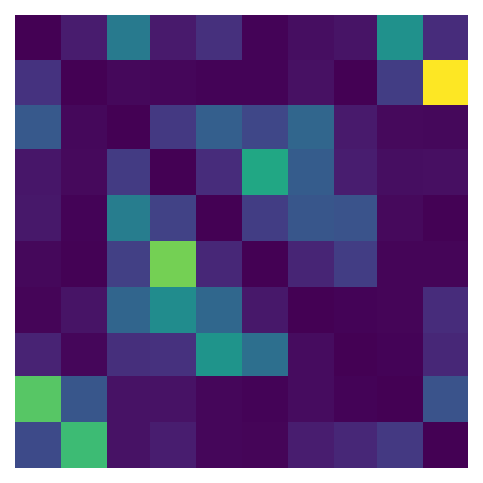
\includegraphics[width=.7\textwidth]{titlefigure.pdf}
		\vspace{50pt}\\
		\textbf{\Huge Adversarial Label Flips}
		\vspace{40pt}\\
		\textbf{\Large Matthias Dellago \& Maximilian Samsinger}\vspace{20pt}\\
		{\large\today}



	\end{center}
\end{titlepage}

	\DeclarePairedDelimiter\abs{\lvert}{\rvert}%
	\DeclarePairedDelimiter\norm{\lVert}{\rVert}%
	\DeclarePairedDelimiter\ceil{\lceil}{\rceil}
	\DeclarePairedDelimiter\floor{\lfloor}{\rfloor}

\begin{abstract}
	%sell it to sb looking for something good to read.
	%only 4 sentences or so.

	Given a neural network (NN) trained to classify, and an untargeted evasion attack, in what class does the adversarial example fall post-attack?
	In the following, we will answer this question by evaluating some state of the art attacks on a simple NN trained on industry standard datasets.
	We discover that intuitively similar classes are more likely to be confused with another, leading us to hypothesise that the NN recognises these similarities.
\end{abstract}

\section{Introduction}

%Adversarial examples exist.
%Targeted and untargeted.
%What does that look like?
%We use confusion matrices.
%example.
%how did we do it? -> NN + foolbox + mnist cifar (section methods)
%what did we get out of it? -> symmetric matrices and interesting insight about noise. (section results)


In 2013 Szegedy et al. demonstrated that deep neural networks (NN) are susceptible to attacks \cite{Szegedy13}. These adversarial examples consist of a small perturbation applied to a otherwise innocuous input, engineered to cause the NN to misbehave.

In our case, the inputs will be images and the attack will be small changes to said image, designed to cause the classifier NN to misclassify the target.

These attacks on classifiers come in two different variations: targeted and untargeted.
In targeted attacks \cite{??} the attacker aims to have the adversarial example identified as a specific class by the NN. (Say, misclassify a dog as a cat.)
An untargeted attack \cite{??} meanwhile, only tries to evade correct classification. (Make this dog appear as anything, apart from a dog.)

When considering untargeted attacks, the question what the adversarial image is classified as post-attack naturally arises. This is what we will experimentally answer in this paper.

\begin{figure}[h]
	\begin{tabular}{cc|c|c|c|}
		& \multicolumn{1}{c}{} & \multicolumn{3}{c}{are categorised as}\\
		& \multicolumn{1}{c}{} & \multicolumn{1}{c}{Dog}  & \multicolumn{1}{c}{Cat} & \multicolumn{1}{c}{Plane} \\\cline{3-5}
		\multirow{3}*{Adversarial examples of a}  & Dog & 2 & 6 & 2\\\cline{3-5}
		& Cat & 7 & 3 &  0 \\\cline{3-5}
		& Plane & 1 & 2 &  7 \\\cline{3-5}
	\end{tabular}

	\caption{An example of a confusion Matrix. Unsuccessful attacks (along the diagonal) are also included.}
	\label{fig:matrixexample}
\end{figure}

We will present our results in terms of confusion matrices. In figure \ref{fig:matrixexample} you can see an example. In larger matrices numbers become more difficult to grasp, so we will display our results in heatmap-style images, as seen on the title page.

In our experiments (Section \ref{sec:experiments}) we used the foolbox framework \cite{rauber2017foolbox}, and simple NNs trained on the MNIST~\cite{deng2012mnist}, Fashion-MNIST~\cite{deng2012mnist} and CIFAR-10~\cite{krizhevsky2009learning} datasets. We applied three state of the art attacks: Projected Gradient Decent (PDG)\cite{madry2017towards}, Carlini-Wagner \cite{carlini2017towards} and Brendel-Bethge\cite{brendel2019accurate}.

We show that, for the CIFAR-10 dataset the confusion matrices are surprisingly symmetric, and intuitively similar classes are often confused with each other. Furthermore we observe that for attacks which are allotted a large perturbation budget, there exist certain attractor classes, which most of the adversarial images are classified as. (Section \ref{sec:results})

%\\
%
%what is our contribution. (we show that these confusion matrix are surprisingly nonrandom)
%\\
%use forward references i.e. "we elaborate on this in sectrion 4".\\
%Give an example for a confusion matrix straight away.



\section{Background and related work}

\paragraph{Existence of adversarial examples}
Since being first demonstrated \cite{Szegedy13} a large body of literature has flourished around adversarial examples. We in the following we will briefly introduce the attacks we use.

%\paragraph{Notions of similarity}
%As mentioned previously we want to fool the NN with a small perturbation, that is to say a image which is very similar. But what do we precisely mean by "small perturbation" and "similar"? We could argue that an image with only one pixel changed is very similar, but also that an image in which each pixel was altered only very slightly is similar.
%
%These different intuitive notions of distance and similarity are captured by different norms.
%
%The distance of two images ($x$,$y$) (i.e. vectors) is described by a metric $D$. This metric can be defined via different norms, most commonly the $L^\infty$-, $L^1$- and $L^2$-norms.( The $L^0$-"norm" is also frequently used, though not a norm in the strict sense.) The distance between these the two images, is then defined as the $L^p$-norm of their difference, for a given $p$:
%
%\begin{equation}
%D(x,y) \defneq \norm{y-x}_p % Here the := is fixed and i created a command for the norm. Hope that helps!
%\end{equation}
%\begin{equation}
%D(x,y) := \| y - x \|_p % Previous version for reference
%\end{equation}
%
%
%\textbf{... Hmmm probably not that important, maybe if there is time and space after everything else in finished.}

\subsection{Attacks}\label{sec:Attacks}

\paragraph{Fast gradient sign method}
Goodfellow et al. seminally developed the fast gradient sign method (FGSM) \cite{goodfellow2014explaining}, making attacks fast and easy. Its key insight was that the backpropagation commonly used to update the weights and biases can be applied all the way back to the input data itself to yields the gradient of the cost function. They then apply gradient decent to find an adversarial example. Since they optimise for the $L^\infty$-norm, all entries of the perturbation are scaled to the same magnitude.

\paragraph{Projected gradient descent}
Projected gradient descent (PGD) was first shown in \cite{madry2017towards}. Conceptually it is very similar to iterating FGSM until converging in a local misclassification optimum. The "projected" part of the name, derives from the fact that upon leaving a ball of radius $\epsilon$ instead of continuing iteration, they project back onto said ball. From iterated FGSM resumes.
This attack leads to formidable results, especially using the $L^\infty$-norm.


% Their experiments suggest that these attacks converge, i.e. they find a local maxima. This may require some restarts.

\paragraph{Carlini-Wagner attack}

Carlini and Wagner \cite{carlini2017towards} invented a different style of attack, where the cost function of the classifier and the distance of the adversarial example are wrapped into one function. They can then simultaneously optimise for both using the Adam stochastic optimiser \cite{kingma2017adam}.

\paragraph{Brendel-Bethge attack}

Brendel and Bethe invented a quite different approach~\cite{brendel2019accurate}.
Their method works by starting from a image deep inside the misclassification region and then preforming binary search between it and the benign, target image, to find the decision boundary. Once there, they move along the boundary to minimise the distance to the benign image, yielding a powerful adversarial example.

\paragraph{Foolbox}
Foolbox is a convenient python toolbox for generating adversarial examples~\cite{rauber2017foolbox}. It supports a large collection of attacks, including all of the above.

\subsection{Quantifying Symmetry}

Since we found a surprising amount of symmetry in the confusion matrices (Section \ref{sec:results}), we wanted to somehow quantify exactly \textit{how} symmetric our matrices were. Upon a review of the literature we could not find any such metric, and so we decided to improvise our own.

Given the confusion matrix $A$ we first replace the diagonal values with zero, since these only represent failed attacks, to get $A_0$. We then split $A_0$ into its symmetric and anti-symmetric constituent matrices:

\begin{equation}
	A_{sym} = \frac{A_0 + A_0^T}{2}, \qquad
	A_{anti} = \frac{A_0 - A_0^T}{2}
\end{equation}

We then define our measure for symmetry $s$:

\begin{equation}
	s = \frac{ \|A_{sym}\|_1 - \|A_{anti}\|_1}{\|A_{sym}\|_1 + \|A_{anti}\|_1}
\end{equation}

(The 1-norm is not special, and could be replaced with any other $p$-norm.)

For confusion matrices (i.e. all values $a_{ij}$ greater zero) $s$ can take values from $[0,1]$. $s = 1$ represents maximally symmetric matrices, and $s = 0$ a maximally skewed matrix.

Below are some examples, to aid our dear reader in building an intuition.

\begin{equation*}
	s\bigg(\begin{bmatrix}
		0 & 1 \\
		0 & 0
	\end{bmatrix}\bigg) = 0, \qquad
%
	s\bigg(\begin{bmatrix}
		0 & 1 \\
		1 & 0
	\end{bmatrix}\bigg) = 1, \qquad
%
	s\bigg( \begin{bmatrix}
		0 & 1 \\
		0.5 & 0
	\end{bmatrix}\bigg) = 0.5
\end{equation*}
%\subsection{Neural networks (Necessary)}
%Is this section necessary? It seems that whoever is interested in our results, easily already knows this.
%\texttt{No, we can just mention neural networks in the introduction and specify our models in the experiments section}
%
%First introduced in \cite{lecun1999object}. The authors of
%\cite{krizhevsky2012imagenet} demonstrated the effectiveness of deep convolutional neural networks on ImageNet.
%
%\paragraph{ResNets}
%Paradigm shift in deep learning. In \cite{he2016deep} they developed Residual Networks to train very deep neural networks. We will probably use ResNet18. If we do, we probably also cite \cite{he2016identity} for the "pre-activation" optimization. This is just a better architecture obtained by having BatchNorm-ReLU-Weights blocks instead of Weights-BatchNorm-ReLU blocks.



\section{Experiments}
\label{sec:experiments}

In this Section we use the adversarial attacks introduced in Section~\ref{subsec:attacks} to compute adversarial examples on the MNIST~\cite{deng2012mnist}, Fashion-MNIST~\cite{xiao2017fashion} and CIFAR-10~\cite{krizhevsky2009learning} datasets. Each dataset is split into a training and test set and all adversarial attacks are computed and evaluated on the test set. Given a dataset and an attack we generate a pair of labels containing the original class and the predicted class for each adversarial example. We use $i$ to denote the $i$-th original class and $j$ to denote the $j$-th predicted class. Since all three datasets contain 10 classes each we obtain $10\times10$ confusion matrices
\[A=(a_{ij})_{\begin{subarray}{l} 1\le i\le 10 \\ 1\le j\le 10\end{subarray}},\]
where $a_{ij}\in\mathbb{N}$ corresponds to the total number of occurrences of each pair $(i,j)$.


\subsection{Experimental setup}
All experiments are conducted in Python 3.8.5~\cite{van1995python} using the PyTorch 1.8.1~\cite{pytorch} library on a Windows machine. Adversarial attacks are computed using FoolBox 3.3.1~\cite{rauber2017foolbox}. Each attack is instantiated using the FoolBox default parameters. All minimization attacks, i.e. \texttt{L0BrendelBethgeAttack}, \texttt{L1BrendelBethgeAttack}, \texttt{L2CarliniWagnerAttack} have their perturbation budget \texttt{epsilons} set to \texttt{None}. This prevents any early termination; a fixed number of iterations is used to compute the adversarial example with minimal perturbation size. For \texttt{LinfPGD} we set \texttt{epsilons} to one of the values in $[0.01, 0.02, 0.05, 0.1, 0.2, 0.5, 1]$ to cover a wide range of perturbation budgets.

\noindent Reference to figures.

\paragraph{Reproducability}All our code, figures and the models we trained are available on GitHub \footnote{\url{https://github.com/MXSMCI/AdversarialLabelFlips}}.

\subsection{Architectures}
We consider the MNIST Model and CIFAR Model, two architectures which are described in \cite{carlini2017towards}, Table 1 and 2. Both architectures consist of two blocks of Convolutional-Convolutional-MaxPooling layers followed by three fully connected layers. All but the last layer use ReLU \cite{maas2013rectifier} as its activation function, whereas the final layer uses the softmax function.\\
One author of \cite{carlini2017towards} provides a reference implementation available on GitHub \footnote{\url{https://github.com/carlini/nn_robust_attacks}}. We achieved similar results in terms of accuracy with our PyTorch reimplementation and can therefore confirm the validity of their results.  \\
For our experiments on the MNIST and Fashion-MNIST dataset we use the MNIST model. For the CIFAR-10 dataset we use the CIFAR Model.

\section{Results}
\label{sec:results}
Here we present all the confusion matrices we calculated. We add our symmetry score as well as the epsilon value, if applicable.



% Eine for loop in latex, wir sind jetzt bei den cool kids, Max!
\foreach \n in {CIFAR-10, FashionMNIST, MNIST}
{
	\subsection{\n}
		%\subsubsection{$L^2$-Carlini-Wagner}
		\begin{figure}[H]
			\centering
			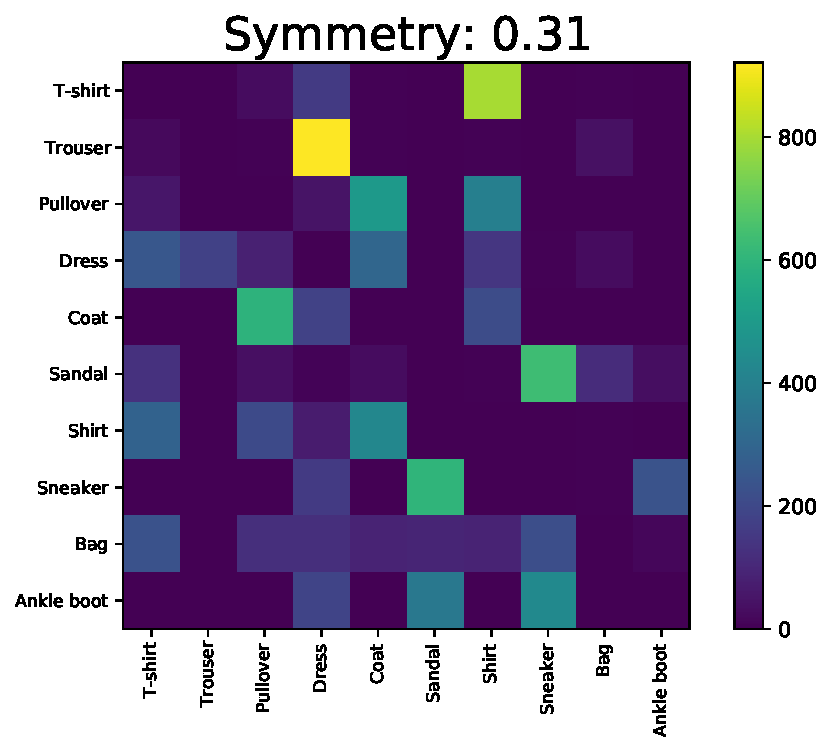
\includegraphics[width=0.5\textwidth]{../code/results/\n/figures/L2CarliniWagnerAttack.pdf}
			\caption{$L^2$-Carlini-Wagner-Attack on \n}
			\label{fig:\n-C-W}
		\end{figure}
	%\subsubsection{Brendel-Bethge}

	\begin{figure}[H]
		\centering
		\begin{subfigure}[b]{0.4\textwidth}
			\centering
			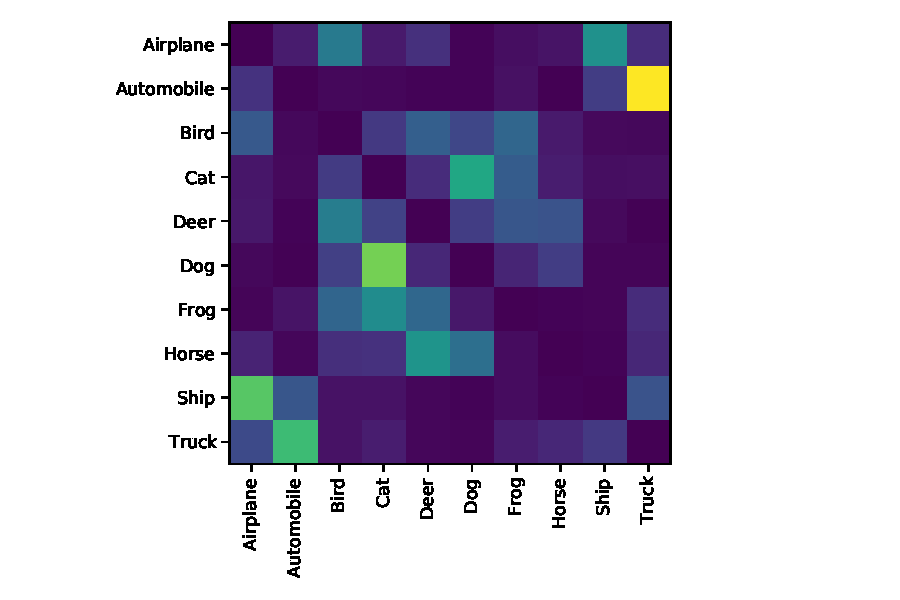
\includegraphics[width=\textwidth]{../code/results/\n/figures/L0BrendelBethgeAttack.pdf}
			\caption{$L^0$}
			%\label{fig:y equals x}
		\end{subfigure}
		\hfill
		\begin{subfigure}[b]{0.4\textwidth}
			\centering
			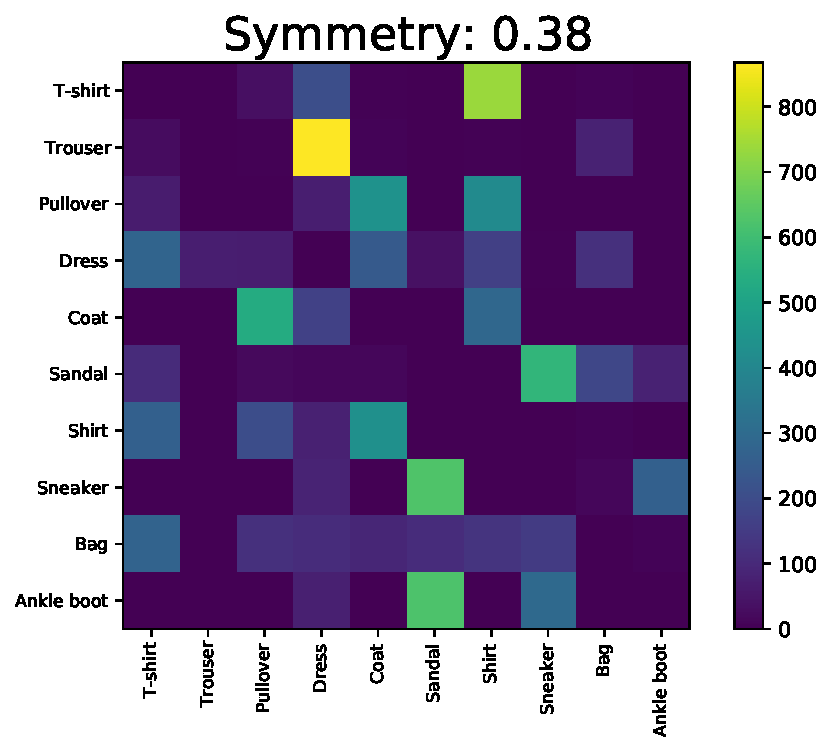
\includegraphics[width=\textwidth]{../code/results/\n/figures/L1BrendelBethgeAttack.pdf}
			\caption{$L^1$}
			%\label{fig:}
		\end{subfigure}
		\caption{Brendel-Bethge-Attacks on \n}
		\label{fig:\n-B-B}
	\end{figure}

	%\subsubsection{$L^\infty$-PGD}
	\begin{figure}[H]
		\begin{tabular}{cccc}
			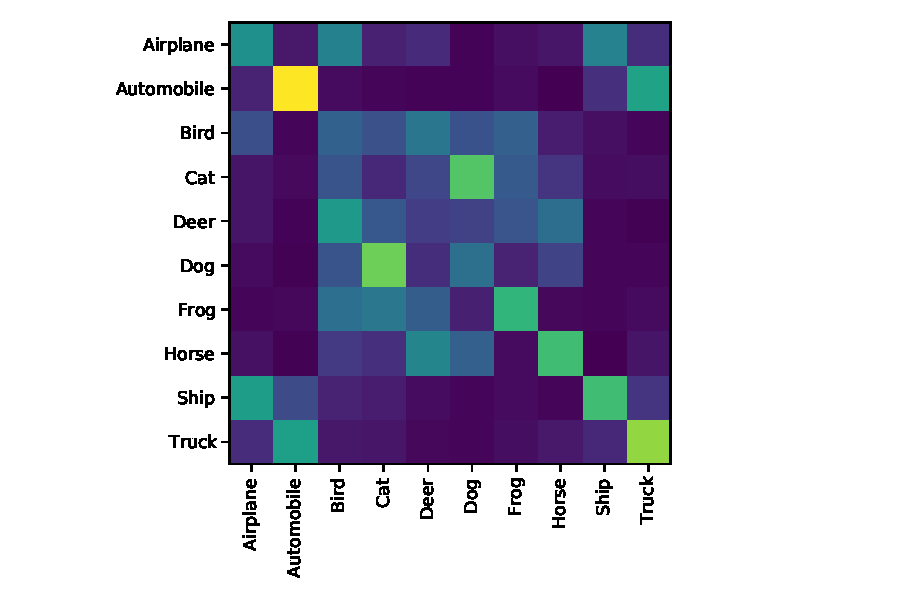
\includegraphics[width=0.3\columnwidth]{../code/results/\n/figures/LinfPGD, epsilon=0.01.pdf} &
			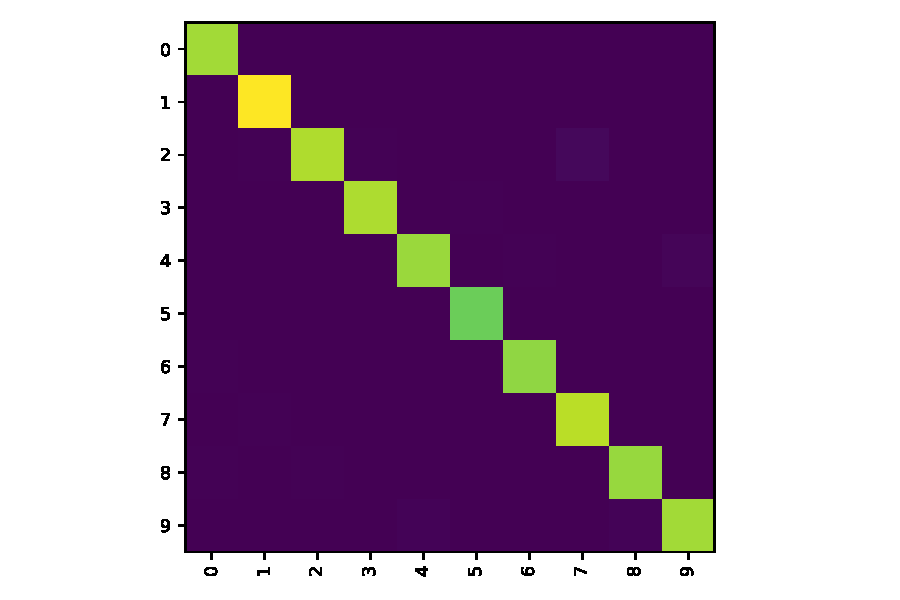
\includegraphics[width=0.3\columnwidth]{../code/results/\n/figures/LinfPGD, epsilon=0.02.pdf} &
			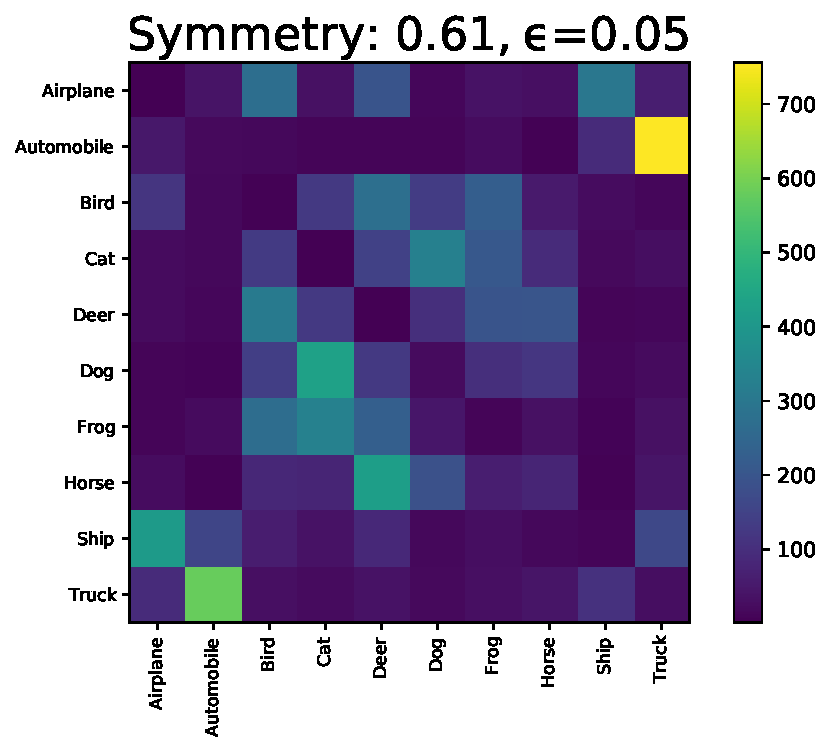
\includegraphics[width=0.3\columnwidth]{../code/results/\n/figures/LinfPGD, epsilon=0.05.pdf} &
			\bigskip \\

			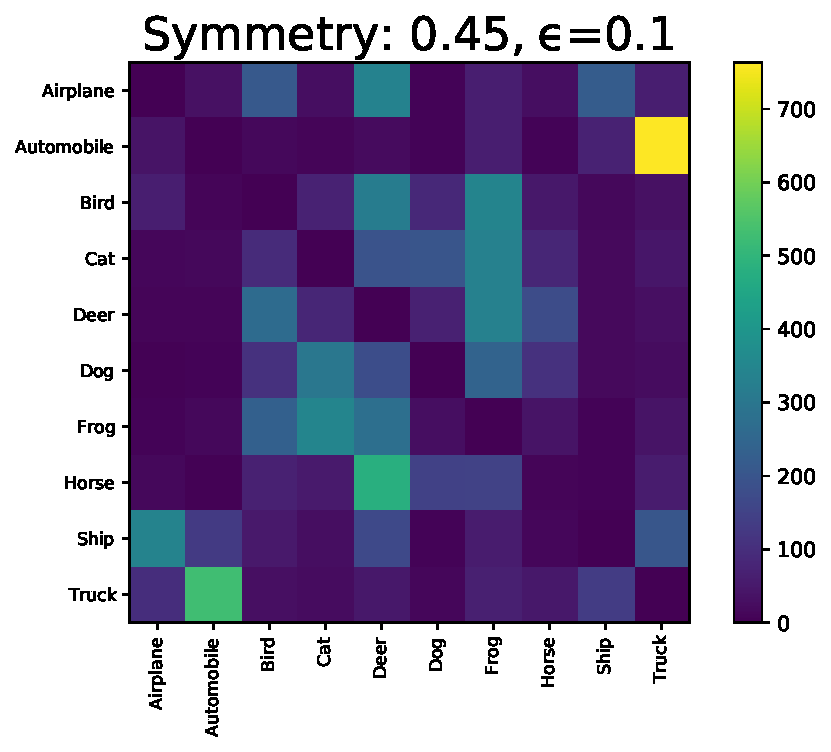
\includegraphics[width=0.3\columnwidth]{../code/results/\n/figures/LinfPGD, epsilon=0.1.pdf} &
			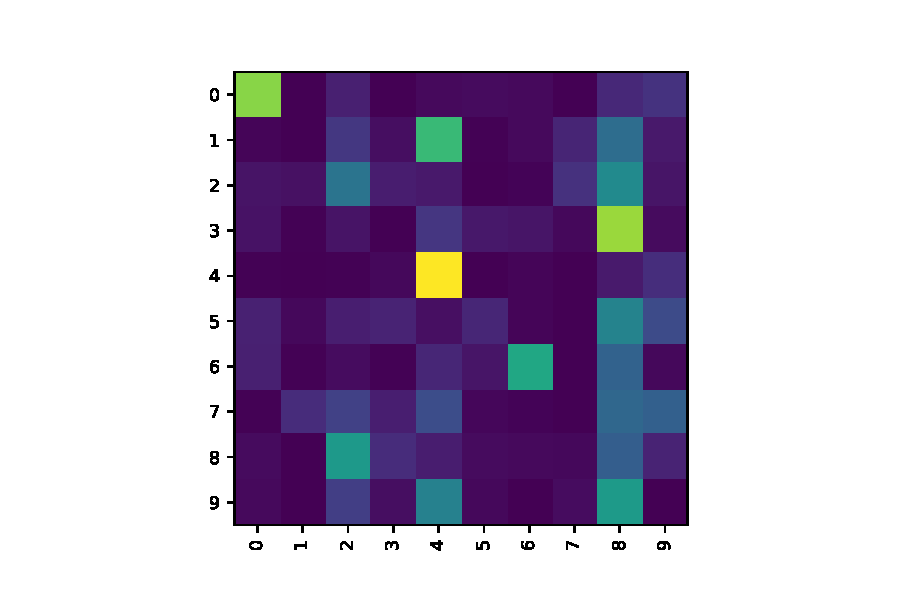
\includegraphics[width=0.3\columnwidth]{../code/results/\n/figures/LinfPGD, epsilon=0.2.pdf} &
			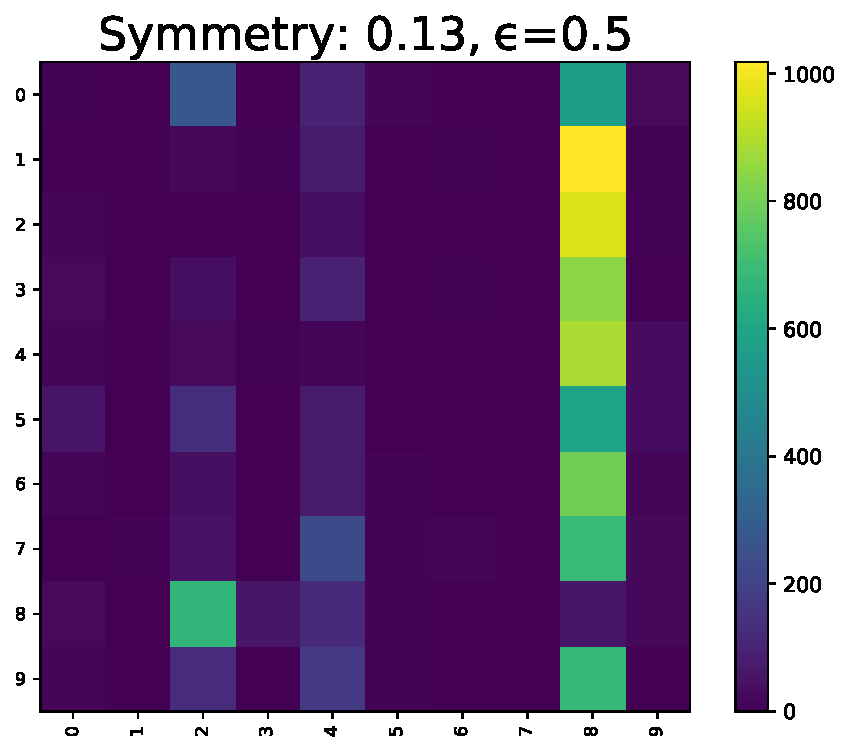
\includegraphics[width=0.3\columnwidth]{../code/results/\n/figures/LinfPGD, epsilon=0.5.pdf} &
		\end{tabular}

		\caption{$L^\infty$-PGD-Attack on \n}
		\label{fig:\n-PGD}
	\end{figure}

}


\section{Discussion}

\paragraph{Symmetry}
Probably the most notable feature of our results is the high degree of symmetry of the CIFAR-10 confusion matrices (Figures \ref{fig:CIFAR-10-C-W}, \ref{fig:CIFAR-10-B-B}, \ref{fig:CIFAR-10-PGD}). This means that, the NN that learned to classify CIFAR-10 is equally likely to mistake class $i$ as class $j$ as the other way around ($j$ as $i$).

Upon taking a closer look at the classes that are likely to be mistaken for another, our reader may notice a pattern. Across the board, the two most common causes of confusion are the pairs "Automobile"-"Truck", and "Dog"-"Cat". From a human perspective, this is a understandable mistake; these two categories are in fact similar in appearance. The other matrix entries follow a similar pattern, with confusions amongst animals and vehicles, being significantly more common than across these two categories.

It therefore seems that the NN captures some notion of similarity, that is quite close to what a human would intuit.
\vspace{12pt}


The MNIST, and FashionMNIST dataset do not appear to match this hypothesis too well.

In Figures \ref{fig:FashionMNIST-C-W} and \ref{fig:FashionMNIST-B-B} the FashionMNIST-NN appears prone to confusing the pairs "Sandals"-"Sneakers" and "Coat"-"Pullover", but adversarial examples of Dresses are far more likely to be classified as "Trouser" than vice versa. The PGD-Matrices (Fig. \ref{fig:FashionMNIST-PGD}) have quite high symmetry scores, but nothing particularly captures the eye.

The MNIST confusion matrices yield comparatively low symmetry scores (Fig. \ref{fig:MNIST-C-W}, \ref{fig:MNIST-B-B}, \ref{fig:MNIST-PGD}). We propose that this is due to a overpowered NN and resulting overfitting. \textbf{Passt das von dir aus Max?}


\paragraph{Catch-all Class} In Figures \foreach \j in {CIFAR-10, FashionMNIST, MNIST}{\ref{fig:\j-PGD}, }one can observe that adversarial examples computed with large perturbation budgets $\epsilon$ are misclassified as "8", "TODO" and "frog" for MNIST, Fashion-MNIST and CIFAR-10 respectively. In order to shed light onto this phenomenon we generate and classify $10000$ white noise images sampled from a uniform distribution on the input domain. Figure A shows that these randomly generated images are also, most commonly, classified as "8", "TODO" and "frog" respectively. This result suggests that the neural networks in question have a default output for low probability images with respect to distribution of the input domain, which in turn affects adversarial examples computed with large perturbation budgets.



\section{Conclusion}
We explored confusion matrices generated by many common untargeted attacks, and discovered interesting structure.
They are decidedly non-random in at least two ways:
\begin{itemize}
	\item Adversarial images which come very close to the original image (e.g. small $\epsilon$) can yield surprisingly symmetric confusion matrices. This symmetry means that class $i$ is confused with class $j$ about as often as vice versa. To us this indicates, that the NN has learned that some classes are more closely related than others.
	This idea is corroborated by the fact that, in these cases the NN confuses semantically similar images in a rather intuitive fashion; for instance confusing "horses" with "deer", and "automobiles" with "trucks".

	\item Attacks which are given a more generous $\epsilon$ tend to cluster into one specific class ("frog" and "8"). We hypothesised that this is due the NN using this class as a catch-all for all images it has difficulty classifying. Using a large batch of noise images we were able to confirm this hypothesis.
\end{itemize}

\section{Contribution Statement}

This is joint work from Maximilian Samsinger and Matthias Dellago. Max trained the NN and evaluated the attacks, Matthias wrote most of the paper. \textbf{Passt das so? Soll noch was rein?}
We thank Alexander Schlögl for the research idea.
\bibliographystyle{unsrt}
\bibliography{literature}

\appendix
\newpage
\section{Figures}

\end{document}
